\documentclass[annotation,times]{itmo-student-thesis}
\usepackage{tikz}
\usepackage{graphicx}
\usepackage{placeins}
\graphicspath{{images/}}
\usetikzlibrary{arrows}
\usepackage{filecontents}

\addbibresource{bachelor-thesis.bib}

\begin{document}
	
	\studygroup{M3436}
	\title{Разработка параллельного алгоритма недоминирующей \\ сортировки}
    \author{Ким Анатолий Валерьевич}{Ким А.В.}
    \supervisor{Буздалов Максим Викторович}{Буздалов М.В.}{канд. техн. наук}{доцент кафедры КТ}
	\publishyear{2017}

    % Здесь должны быть даты (сдача, защита)

    %%% Цель исследования
    \researchaim{Целью данной работы является получение эффективного параллельного алгоритма 
                 недоминирующей сортировки на основе имеющихся решений.}

    %%% Задачи, решаемые в ВКР
    \researchtargets{\begin{enumerate}
        \item анализ существующий решений;
        \item разработка эффективного параллельного алгоритма;
        \item экспериментальное исследование эффективности полученного решения;
    \end{enumerate}}

    %%% Использование современных пакетов компьютерных программ и технологий
    \advancedtechnologyusage{Алгоритм был разработан на языке программирования Java.}

    %%% Краткая характеристика полученных результатов 
    \researchsummary{Был разработан алгоритм.}

    %%% Гранты, полученные при выполнении работы 
    \researchfunding{Гранты отсутствуют.}

    %%% Наличие публикаций и выступлений на конференциях по теме выпускной работы
    \researchpublications{Данная работа не имеет публикаций.}
	
	%% Эта команда генерирует титульный лист и аннотацию.
    \maketitle{Бакалавр}

	%% Оглавление
	\tableofcontents
	
    \startprefacepage
Большинство многокритериальных эволюционных алгоритмов использует оптимальность в смысле Парето в качестве критерия отбора решений. Процедура многокритериальной оптимизации в этих алгоритмах как правило доминирует в общей временной сложности одной итерации. По этой причине ускорение данной процедуры является ключом к более эффективным многокритериальным эволюционным алгоритмам.

В случае с оптимальностью по Парето, задачей многокритериальной оптимизации является задача недоминирующей сортировки. На сегодняшний день существует несколько алгоритмов недоминирующей сортировки с различной асимптотической сложностью и реальным временем работы. Их эффективность сильно зависит от специфики входных данных.
 
Целью данной работы является разработка эффективного параллельного алгоритма недоминирующей сортировки на основе имеющихся решений.

	
    \chapter{Обзор предметной области}
В этой главе описываются основные понятия и термины предметной области, к которой относится представленная работа. Также проводится обзор имеющихся алгоритмических решений и формулируется постановка задачи.

\section{Основные определения}

Принципиальное отличие многокритериальных задач оптимизации от однокритериальных заключается в том, что во втором случае целью является поиск самого оптимального решения. В случае же задачи многокритериальной оптимизации такого решения может не существовать вследствие возможных конфликтов целевых функций. Таким образом, многокритериальная оптимизация основывается на компромиссном поиске группы оптимальных решений в смысле Парето.
\begin{definition}
    В $M$-мерном пространстве, точка $A = (a_1, \ldots, a_M)$ доминирует в смысле Парето точку $B = (b_1, \ldots, b_M)$, когда для всех $1 \leq i \leq M$ выполняется неравенство $a_i \leq b_i$ и существует хотя бы одно такое $j$, что $a_j < b_j$.
\end{definition}
\begin{definition}
    Недоминирующая сортировка множества точек $S$ в $M$-мерном пространстве --- это процедура, в процессе которой всем точкам, которые не доминируются никакими другими точками, назначается ранг $0$. Далее всем точкам, которые доминируются только точками с рангом $0$, назначается ранг $1$, и т.д. Все точки с рангом $i$ доминируются только точками с рангом не более $i + 1$.
\end{definition}

\section{Обзор существующих алгоритмов}
\subsection{Тривиальный алгоритм}
Рассмотрим самую наивную версию алгоритма недоминирующей сортировки. Найдем все недоминируемые точки с нулевым рангом, вычеркнем эти точки и будем повторять эту процедуру, каждый раз назначая ранг на единицу больше, чем на предыдущей итерации. Тогда, если $M$ --- количество критериев отбора или размерность множества точек (решений), а $N$ --- количество решений, нам необходимо за время $O(MN^2)$ сравнить $O(N^2)$ пар точек по каждому из $M$ критериев и повторить эту процедуру в худшем случае $N$ раз. Таким образом получаем время работы $O(MN^3)$.

Кунг и др. в своей работе предложили алгоритм поиска недоминируемых решений со сложностью $O(N\log^{M-1}N)$. Совместив предложенный алгоритм с идеей удаления найденных точек, описанной в наивном алгоритме, мы получаем алгоритм недоминирующей сортировки с общей сложностью $O(N^2\log^{M-1}N)$ в худшем случае, если максимальный ранг решений --- $O(N)$.

\subsection{Быстрая недоминирующая сортировка}
Деб в своей работе предложил алгоритм <<Быстрой недоминирующей сортировки>>, улучшив асимптотическую сложность алгоритма до $O(MN^2)$. Этот алгоритм является базисным с точки зрения эффективности в семействе алгоритмов <<Разделяй и властвуй>>.

Йенсен был первым, кто предложил алгоритм недоминирующей сортировки со сложностью $O(N\log^{M-1}N)$, позволив тем самым эффективно вычислять ранги точек для типичных конфигураций входных значений. Однако его алгоритм имел существенный недостаток: он работал корректно только в предположении, что никакие два решения не имеют одинаковых значений по одному и тому же критерию. Фанг и др. в своей работе пришли к заключению, что алгоритм Йенсена неспособен генерировать такие же недоминирующие фронты точек, как оригинальный алгоритм NSGA-II. Также они продемонстрировали, что устранение главного недостатка алгоритма Йенсена является нетривиальной задачей.

Решение данной проблемы было предложено Фортеном и др. Предложенный им <<обобщенный>> алгоритм недоминирующей сортировки работает корректно на любых входных данных, сохраняя при этом среднюю временную сложность $O(N\log^{M-1}N)$. Тем не менее было доказано, что в худшем случае время работы алгоритма составляет $O(N^2M)$.

Дальнейшее улучшение недоминирующей сортировки Фортена было предложено Буздаловым и др. В своей работе он модифицирует алгоритм и доказывает оценку $O(N\log^{M-1}N)$ для худшего случая.

\section{Описание алгоритма <<Разделяй и властвуй>>}

	%\chapter{Реализация алгоритма}
\section{Предлагаемая схема параллелизации}
Две основные процедуры в алгоритме Фортена с модификацией Буздалова --- $NDHelperA$ и $NDHelperB$. Процедура $NDHelperA$ делит задачу на подзадачи и сливает результаты воедино посредством $NDHelperB$. Процедура $NDHelperB$ сама по себе является рекурсивной, следующей парадигме <<разделяй и властвуй>>. Деление задач происходит до момента, когда размерность $k$ станет равна $2$, что в дальнейшем обрабатывается отдельными процедурами.

Можно заметить, что на момент вызова процедуры $NDHelperB(L, H, k)$ ранги точек из множества $L$ уже вычислены и в дальнейшем меняться не будут. Также заметим, что порядок вызова подзадач в теле $NDHelperB$ не нарушит корректности алгоритма. Более того, мы можем разделить множество $L$ на любое количество частей ${L_1, L_2,\ldots, L_n}$ и тогда результат исполнения $NDHelperB(L_i, H, k)$ для всех $i$ будет идентичен результату исполнения $NDHelperB(L, H, k)$. Таким образом, $NDHelperB$ допускает параллельное исполнение.

С параллелизацией процедуры $NDHelperA$ возникают сложности. Внутренние вызовы $NDHelperA$ и $NDHelperB$ зависят друг от друга и имеют строго определенную последовательность. 

\section{Детали реализации}
Алгоритм был реализован на языке программирования Java с использованием Fork/Join фреймворка, который хорошо подходит для распараллеливания рекурсивных задач.


	%\chapter{Реализация и экспериментальное исследование}
\section{Реализация алгоритма}
Алгоритм был реализован на языке программирования Java с использованием фреймворка Fork/Join, который хорошо подходит для параллельного исполнения рекурсивных задач.

\subsection{Используемые алгоритмы и структуры данных}
Входной двумерный массив точек остается неизменным, все операции перестановок и модификаций осуществляются на массивах индексов, чтобы избежать лишних копирований памяти.

Для нахождения медианного значения заданного критерия по всем входным точкам используется алгоритм <<Median of medians>> с линейным временем работы.

Большинство процедур в алгоритме изменяют порядок элементов во входном массиве индексов, в связи с чем в параллельной версии возникает задача изолирования памяти.

При каждом вызове \textsc{NDHelperB} копируется нужный отрезок входного массива индексов.
Для восстановления лексикографического порядка во входном массиве используется операция \textsc{merge}.
Операции \textsc{split}, \textsc{merge} и поиск медианы требуют $O(N)$ дополнительной памяти, поэтому они выполняются на буферах, локальных для каждого потока.

Для поддержания упорядоченных множеств <<ступеней>> Парето-фронтов в \textsc{SweepA} и \textsc{SweepB}, описанных в алгоритме Фортена, были реализованы красно-черное дерево и дерево Фенвика.

Начальная лексикографическая сортировка точек осуществляется с помощью сортировки слиянием.
По мере выполнения лексикографической сортировки заполняется вспомогательный массив $eqComp$ со следующим свойством: если точка $S_i$ совпадает в каждой координате с точкой $S_j$, то $eqComp[i] = eqComp[j]$, если $S_i$ лексикографически меньше $S_j$, то $eqComp[i] < eqComp[j]$.
Эта структура позволяет в дальнейшем сравнивать точки за $O(1)$.

\subsubsection{\textsc{NDHelperA}}
Для реализации описанной во второй главе модификации процедуры \textsc{NDHelperA} необходимо ввести дополнительную структуру, представляющую контекст для отложенного исполнения \textsc{NDHelperB}.

\begin{lstlisting}[float=!h,caption={Вспомогательная структура <<контекст>> для \textsc{NDHelperA}}]
class Context {
    int k;
    int[] compareWith;
    List<Future> futures;
    ...
}
\end{lstlisting}

Добавим в \textsc{NDHelperA} дополнительный аргумент --- список контекстов для отложенного исполнения \textsc{NDHelperB}.

В каждом таком контексте будет храниться:
\begin{itemize}
    \item размерность $k$, по которой будет производиться сравнение;
    \item список индексов $compareWith$ --- точки, с которыми необходимо сравниться;
    \item список $futures$, в который необходимо положить результат отложенного вычисления \textsc{NDHelperB};
\end{itemize}

Если входящий список контекстов не пуст, то до завершения работы \textsc{NDHelperA} необходимо асинхронно запустить выполнение \textsc{NDHelperB} на каждой из частей $L$, $M$ и $H$ в паре с точками из каждого контекста, или на входном отрезке целиком, если деление на части не выполняется.

Результат отложенного исполнения необходимо положить в список $futures$, чтобы у нас была возможность дождаться завершения работы в необходимой нам точке.

В \textsc{NDHelperA(L)} помимо контекстов, переданных сверху, добавляется два новых контекста: первый с отрезком $M$ и списком $waitM$, второй --- с отрезком $H$ и списком $waitH$.
В \textsc{NDHelperA(M)} добавляется контекст с $H$ и списком $waitH$.
Перед запуском \textsc{NDHelperA(M)} мы должны дождаться выполнения задач в $waitM$, а перед запуском \textsc{NDHelperA(H)} --- задач в $waitH$.
Таким образом, все требуемые сравнения точек будут завершены к нужному моменту.

\subsection{Переключение на последовательную версию}
Каждый параллельный вызов \textsc{NDHelperB} при использовании $Fork/Join$ влечет за собой накладные расходы, потому что нам нужно создать новый объект для каждой подзадачи, а также скопировать необходимые отрезки индексов.
Поэтому при достаточно маленьких размерах входных массивов имеет смысл запускать однопоточную версию процедуры.

Был проведен ряд экспериментов при $N=\{10^4, 5\cdot10^4, 10^5\}$, $M=\{3,4,\ldots,15\}$.
В качестве порога в \textsc{NDHelperB} рассматривались степени двойки от $4$ до $1024$.

Лучшие результаты были достигнуты при пороге равном $32$.
Таким образом, если $|L| < 32$ или $|H| < 32$, то запускается однопоточная версия \textsc{NDHelperB(L, H, k)}.

\section{Экспериментальное исследование алгоритма}
Далее будут представлены результаты экспериментального исследования эффективности предложенного алгоритма.

Эксперименты проводились на компьютере с шестнадцатиядерным процессором \textit{AMD Opteron(tm) Processor 6380} с частотой 2.5 ГГц и 4 Гб оперативной памяти.

В качестве тестовых данных использовались искусственно сгенерированные массивы случайных значений. 

Каждая версия алгоритма тестировалась на одной конфигурации входных данных и фиксированном числе потоков исполнения по 25 раз, далее сравнивались минимальное, максимальное и медианное время работы.

\subsection{Сравнение с однопоточной версией алгоритма}
По результатам экспериментов видно, что при больших $N$ достигается неплохой уровень параллелизма.
При $M\leq3$ польза от параллельного исполнения отсутствует, т.к. корневые \textsc{NDHelperB} вызываются с $k=2$, т.е. запускается однопоточная процедура \textsc{SweepB}.

С увеличением $M$ растет количество параллельных подзадач \textsc{NDHelperB}, соответственно прирост в производительности становится более заметным.
Начиная с некоторого значения $M$, глубина дерева исполнения \textsc{NDHelperB} определяется значением $N$ и перестает зависеть от $M$, происходит насыщение всех потоков.

\begin{figure}[h!]
\centering
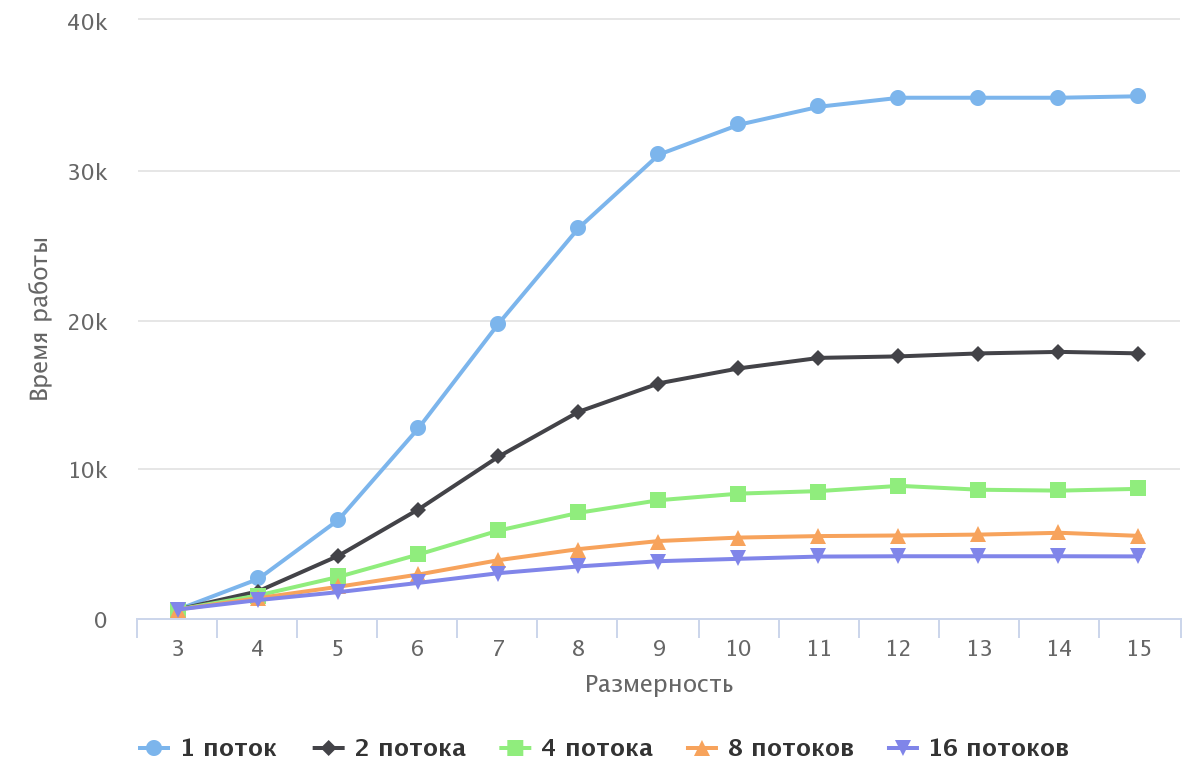
\includegraphics[width=\textwidth]{images/100k.png}
\caption{Медианное время работы\\параллельного алгоритма при $N=10^5$}
\end{figure}

Нам удалось добиться максимального ускорения в $8.47$ раз при $10^5$ точках и 16 потоках.

\begin{table}[h!]
\caption{Время работы алгоритма при $N=10^5$}\label{tab1}
\centering
\begin{tabu}{|*{8}{c|}}
\hline
 & \multicolumn{3}{c|}{Original} & \multicolumn{4}{c|}{Parallel 16 threads}\\
\cline{2-8}
    M & min & max & med & min & max & med & $t_1/t_2$ \\
\hline
    3 & 5.66e+02 & 5.70e+02 & 5.68e+02 & 5.67e+02 & 5.73e+02 & 5.70e+02 & \textbf{1.00}\\ 
    4 & 2.50e+03 & 2.82e+03 & 2.61e+03 & 1.13e+03 & 1.27e+03 & 1.20e+03 & \textbf{2.16}\\
    5 & 6.46e+03 & 6.80e+03 & 6.56e+03 & 1.67e+03 & 1.89e+03 & 1.73e+03 & \textbf{3.79}\\
    6 & 1.26e+04 & 1.28e+04 & 1.27e+04 & 2.28e+03 & 2.45e+03 & 2.35e+03 & \textbf{5.40}\\
    7 & 1.96e+04 & 1.99e+04 & 1.97e+04 & 2.93e+03 & 3.06e+03 & 3.00e+03 & \textbf{6.57}\\
    8 & 2.59e+04 & 2.62e+04 & 2.61e+04 & 3.30e+03 & 3.57e+03 & 3.45e+03 & \textbf{7.57}\\
    9 & 3.08e+04 & 3.12e+04 & 3.10e+04 & 3.69e+03 & 3.91e+03 & 3.80e+03 & \textbf{8.16}\\
    10& 3.28e+04 & 3.32e+04 & 3.30e+04 & 3.85e+03 & 4.03e+03 & 3.96e+03 & \textbf{8.33}\\
    11& 3.41e+04 & 3.45e+04 & 3.42e+04 & 3.99e+03 & 4.24e+03 & 4.11e+03 & \textbf{8.32}\\
    12& 3.46e+04 & 3.51e+04 & 3.48e+04 & 3.98e+03 & 4.25e+03 & 4.13e+03 & \textbf{8.43}\\
    13& 3.46e+04 & 3.51e+04 & 3.48e+04 & 4.00e+03 & 4.36e+03 & 4.13e+03 & \textbf{8.43}\\
    14& 3.46e+04 & 3.50e+04 & 3.48e+04 & 4.01e+03 & 4.43e+03 & 4.13e+03 & \textbf{8.43}\\
    15& 3.47e+04 & 3.52e+04 & 3.49e+04 & 3.95e+03 & 4.25e+03 & 4.12e+03 & \textbf{8.47}\\
\hline
\end{tabu}
\end{table}

\subsection{Сравнение с параллельным алгоритмом Деба}
Для сравнения двух алгоритмов было выбрано относительно небольшое количество точек, т.к. алгоритм Деба из NSGA-II обладает квадратичным временем работы.

По графикам видно, что квадратичный алгоритм лучше масштабируется независимо от $N$. Тем не менее, из-за более плохой асимптотики, он уступает в эффективности предложенному алгоритму при любом количестве потоков от $1$ до $16$. Более того, алгоритм Фортена начинает превосходить шестнадцатипоточный алгоритм Деба уже на четырех потоках.

\begin{table}[h!]
\caption{Сравнение алгоритмов на 16 потоках при $N=10^4$}\label{tab1}
\centering
\begin{tabu}{|*{8}{c|}}
\hline
 & \multicolumn{3}{c|}{Алгоритм Деба} & \multicolumn{4}{c|}{Предложенный алгоритм}\\
\cline{2-8}
    M & min & max & med & min & max & med & $t_1/t_2$ \\
\hline
    3 & 4.80e+02 & 5.03e+02 & 4.91e+02 & 2.69e+01 & 2.72e+01 & 2.70e+01 & \textbf{18.00}\\ 
    4 & 3.29e+02 & 3.83e+02 & 3.53e+02 & 1.16e+02 & 1.41e+02 & 1.34e+02 & \textbf{2.63}\\
    5 & 2.89e+02 & 3.31e+02 & 3.10e+02 & 1.35e+02 & 1.77e+02 & 1.57e+02 & \textbf{1.97}\\
    6 & 2.86e+02 & 3.67e+02 & 3.04e+02 & 1.59e+02 & 2.19e+02 & 1.77e+02 & \textbf{1.72}\\
    7 & 3.07e+02 & 3.89e+02 & 3.23e+02 & 1.65e+02 & 2.19e+02 & 1.86e+02 & \textbf{1.74}\\
    8 & 3.08e+02 & 4.19e+02 & 3.36e+02 & 1.71e+02 & 2.15e+02 & 1.93e+02 & \textbf{1.74}\\
    9 & 3.42e+02 & 3.96e+02 & 3.62e+02 & 1.57e+02 & 2.35e+02 & 1.85e+02 & \textbf{1.96}\\
    10& 3.38e+02 & 4.36e+02 & 3.82e+02 & 1.70e+02 & 2.47e+02 & 1.87e+02 & \textbf{2.04}\\
    11& 3.82e+02 & 5.33e+02 & 4.14e+02 & 1.65e+02 & 2.10e+02 & 1.88e+02 & \textbf{2.20}\\
    12& 3.88e+02 & 4.79e+02 & 4.23e+02 & 1.64e+02 & 2.00e+02 & 1.84e+02 & \textbf{2.30}\\
    13& 4.15e+02 & 4.81e+02 & 4.44e+02 & 1.62e+02 & 2.15e+02 & 1.84e+02 & \textbf{2.41}\\
    14& 4.44e+02 & 5.79e+02 & 4.72e+02 & 1.58e+02 & 2.12e+02 & 1.84e+02 & \textbf{2.57}\\
    15& 4.86e+02 & 5.32e+02 & 5.02e+02 & 1.63e+02 & 2.21e+02 & 1.84e+02 & \textbf{2.73}\\
\hline
\end{tabu}
\end{table}

При большем количестве точек разница в производительности алгоритмов будет прослеживаться более явно из-за разницы в асимптотике и увеличением параллельности нашего алгоритма.

\begin{figure}[h!]
\centering
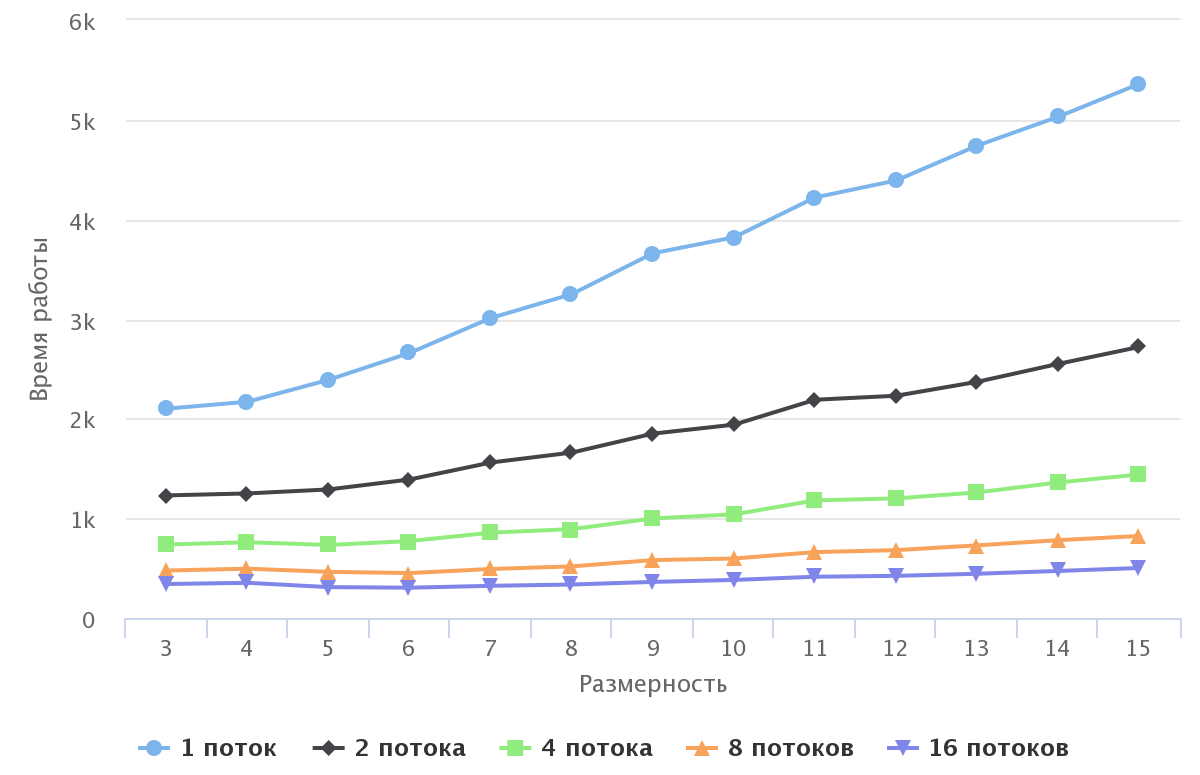
\includegraphics[width=0.95\textwidth]{images/deb10k.png}
\caption{Медианное время работы параллельного алгоритма Деба при $N=10^4$}
\end{figure}

\begin{figure}[h!]
\centering
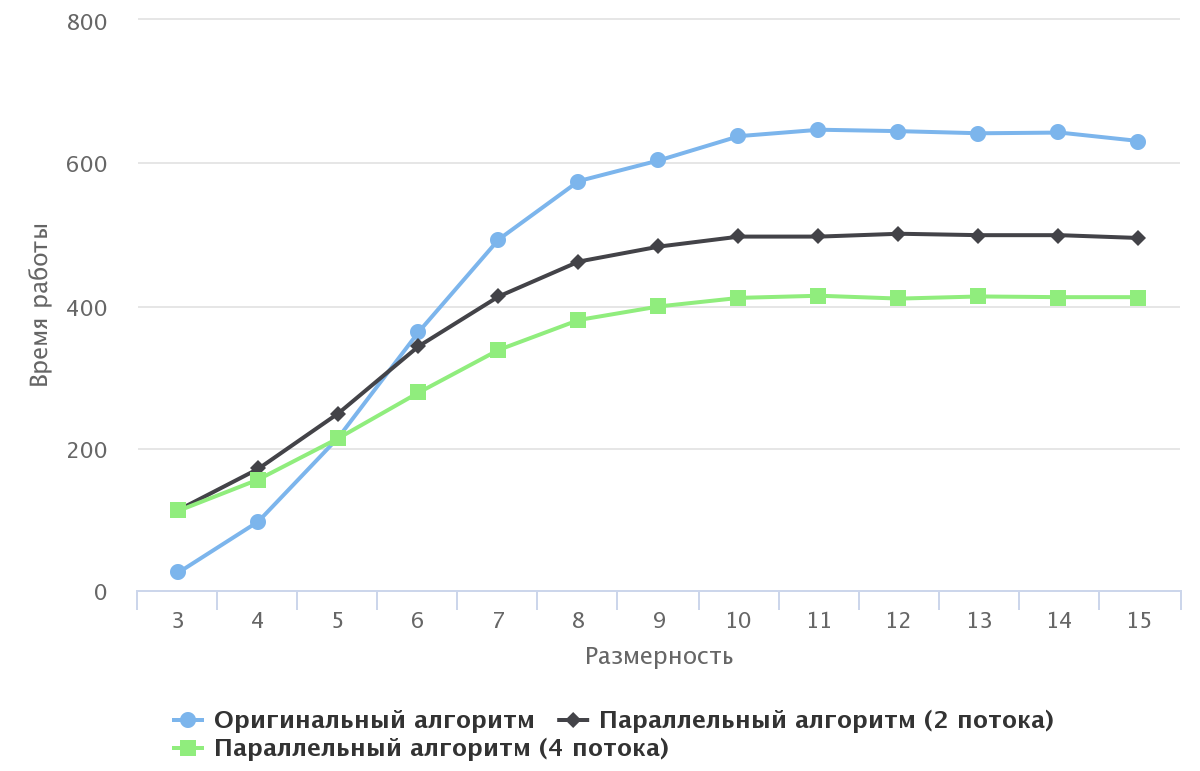
\includegraphics[width=0.95\textwidth]{images/10k.png}
\caption{Медианное время работы параллельного алгоритма Фортена при $N=10^4$}
\end{figure}


	
	%\input{chapters/conclusion.tex}
	
	%\printmainbibliography
	
	%% После этой команды chapter будет генерировать приложения, нумерованные русскими буквами.
	%% \startappendices из старого стилевика будет делать то же самое
	%\appendix
	
	%\chapter{Пример приложения}
	
\end{document}
